\chapter{Fundamentals}
Section \ref{sections:fundamentals/virtualisation} summarises the concept of virtualisation.
Section \ref{sections:fundamentals/namespaces} introduces the concept of a namespace as defined 
in the Linux kernel and describes the individual namespace types and their effects on processes. 
Section \ref{sections:fundamentals/ebpf} presents the benchmarking tool 
that will be used to assess the performance of a namespaced application.

\section{Virtualisation}
\label{sections:fundamentals/virtualisation}
Virtualisation is the process of abstracting the execution environment of an application into 
a unit that is secure, manageable and performant. The primary value propositon of a virtualisation 
platform is the consolidation of independent and untrusted workloads onto a single 
server which cannot interfere with each other or with the host, and still exhibit optimal 
performance characteristics. Virtualisation is, in essence, a cost reduction technique for 
infrastructure providers. Unfortunately, security and performance are concepts that often conflict 
with each other, thereby rendering virtualisation into a particularly challenging domain.

Section \ref{sections:fundamentals/virtualisation/axioms} presents the fundamental axioms 
that define virtualisation - noninterference, isolation, and performance.
The first two axioms will be used to assess the security properties
that namespaces have, while the last one will be used to define a benchmark with metrics that 
measure the performance capabilities of a virtualised application. 

\subsection{Axioms}
\label{sections:fundamentals/virtualisation/axioms}
\subsubsection{Noninterference}
\label{sections:fundamentals/virtualisation/axioms/noninterference}
\textcite{10.1145/368481.368502} summarise the fundamental requirements of a multiprogramming 
system and emphasise the concept of noninterference between processes across space and time. 
\textit{Spatial noninterference} is represented by all mechanisms that protect references to memory, 
disk and input-output devices \cite{10.1145/368481.368502}. For example, memory segmentation 
is a method found in operating system kernels that assigns each process a dedicated portion
of physical memory that is invisible to all other processes in the system. The kernel traps 
any attempt made by a process to access memory outside its allocated memory segment, thereby 
guaranteeing spatial noninterference \cite{10.5555/2490781}. \textit{Temporal noninterference} refers
to those mechanisms that allocate execution time and protect against the monopolisation thereof 
\cite{10.1145/368481.368502}. For instance, CPU scheduling is a technique that decides which process 
shall run on a core such that the core does not idle and all processes make sufficient 
runtime progress \cite{10.5555/2490781}. The scheduling semantics, paired with an interrupt mechanism 
that makes sure that no process has hold of the core for too long, guarantee temporal noninterference.

\subsubsection{Isolation}
\label{sections:fundamentals/virtualisation/axioms/isolation}
\textcite{10.1145/3381052.3381315} define isolation as the level of dependency that a virtualisation 
platform has towards the host kernel. We generalise this definition and say that \textit{isolation} 
is the level of dependency that one piece of software has to another. Conceptually, isolation 
deals with explicit vertical relationships between software, and noninterference deals with 
implicit horizontal relationships between processes. Isolation can be quantified by counting the 
lines of external source code that a software executes to obtain a particular functionality. 
For example, \textcite{10.1145/3381052.3381315} count the lines of kernel code 
that a virtualisation platform executes when providing services to sandboxed applications. 
High counts indicate a strong dependency, i.e weak isolation, towards the kernel. 

\subsubsection{Performance}
\label{sections:fundamentals/virtualisation/axioms/performance}
\textcite{10.1145/3365199} defines performance as the contention between the overhead associated 
with isolating a process from its environment and the benefits of sharing resources between processes,
i.e fully utilising the capacity of the underlying resource pool. 
\textcite{10.1145/3381052.3381315} use the same definition and contrast the isolation mechanisms provided
by three different virtualisation platforms against processing unit, memory and input-output performance metrics. 
In particular, the authors define an application that computes prime numbers up to a limit. 
Since the workload is compute-bound, processing speed is measured and compared to the
number of executed lines of code that reside in the \verb|/arch|, \verb|/virt| and \verb|/arch/x86/kvm|
subsystems of the Linux kernel. \textcite{10.1145/3132747.3132763} use \textit{same-host density} as a 
performance metric that measures the number of sandboxed applications that can be consolidated onto a single server.
In addition, \textit{boot, pause and unpause times} are also considered to be important performance indicators for particular 
use cases, such as elastic content delivery networks \cite{10.1145/3050748.3050757} \cite{10.1145/3132747.3132763}
and serverless computing.

\section{Namespaces}
\label{sections:fundamentals/namespaces}
A namespace encapsulates a system resource and a collection of processes. Only processes that are 
part of the namespace can see and manipulate the resource. Namespaces are implemented in the 
kernel and are therefore a part of the trusted computing base. Container runtimes use them 
to establish a solid noninterference boundary between processes by restricting their view of the system. 
The system calls \verb|clone|, \verb|unshare|, \verb|setns| and \verb|ioctl|, as well as the 
\verb|procfs| pseudo-filesystem are the primary interaction points between a user-space program and a namespace.  

Every process is associated with a fixed-size set of namespaces, called the \textit{namespace proxy}, that corresponds to the
resources that it can access.
In user-space, the proxy is contained within the \verb|/proc/[pid]/ns| directory as a 
collection of symbolic links, each pointing to an inode number uniquely identifying a namespace 
that wraps the process identified by \verb|pid|. Currently, there are seven different types 
of namespaces reflected in the proxy. Each will be discussed individually in the upcoming sections. 

The lifecycle of a namespace is tightly coupled to the lifecycle of all processes that reside in it. 
This is reflected in how namespaces are created and destroyed. 
A namespace and a process can be atomically created via the \verb|clone()| system call.
\verb|clone()| creates a child process that begins its lifecycle by executing 
a function pointer that returns the exit code with which the child process will terminate.
In addition, the caller passes a set of configuration options that define the child's execution context.
The parent can put the child in a freshly-allocated set of namespaces by ORing a set of flags 
and injecting the result into the configuration set. It is important to note that the 
configuration set is very flexible and defines the noninterference boundary between the child and its parent. 
The parent can use it to share its virtual memory pages, file-descriptor table and filesystem information 
with the child, thereby weakening the boundary. 
\verb|unshare()| allows an already existing process to regulate its noninterference boundary by
\enquote{disassociating parts of its execution context}. In other words, a process can 
reverse the configuration options used when it was created.
Hence, the process can detach itself into a new set of namespaces.
Alternatively, \verb|setns()| can be used by a process to join a namespace that already exists. The caller 
must have an open file descriptor referencing a namespace object from the \verb|/proc/[pid]/ns| directory. 
Notice that a namespace cannot be created without having a process to reside in it. 
A namespace is implicitly 
destroyed by the kernel when all processes inside it terminate. 
However, a user-space process can keep a namespace alive by explicitly referencing it through a 
file descriptor obtained from the proxy.

Some namespaces are represented as $n$-ary trees and can be nested up to $32$ times in order to create multiple 
noninterference boundaries. Relationships between namespaces can be queried via the \verb|ioctl|
system call that, in combination with the \verb|NS_GET_PARENT| flag, returns an initialised read-only file descriptor pointing at 
the parent namespace. 

\subsection{User namespace}
\label{sections:fundamentals/namespaces/user}
Every process is associated with a set of credentials. 
The traditional UNIX security model defines these credentials 
as a set of unique numerical user and group identifiers. The \textit{real} user and group identifiers 
represent the user to which the process belongs. They are read from the 
password database as part of the login procedure \cite{10.5555/1869911}. 
Every process spawned by the user inherits the real user and group identifiers as part of 
its credentials. 
The credentials themselves further consist of an \textit{effective} user and an effective group identifier,
which are used by the kernel to authorise and execute operations on behalf of the process \cite{10.5555/1869911}.
For example, when a process attempts to read a file, the kernel checks if the effective user ID
of the process matches the user ID of the owner of the file, or if the effective group ID matches the 
owner's group ID. If any of these predicates holds, then the effective user - and therefore the process - 
is deemed trustworthy to call the \verb|read| system call on a file descriptor referencing the file.
Typically, the effective user and group identifiers match their real counterparts. However, there 
are programs that can ambiently change the effective identifiers of a process to match 
those of the user that created them \cite{10.5555/1869911}. These programs are known as 
\textit{set-user-id} and \textit{set-group-id} programs. Every executable file is associated with 
a set-user-id and a set-group-id permission bit that can be set by that file's owner. 
If the set-user-id permission bit is set and another user executes the program, the process
obtains the effective user identifier of the file's owner, not the user that started the process \cite{10.5555/1869911}.
A classic example of a set-user-id program is \verb|sudo|, which executes arbitrary commands as the 
root user. Since the \verb|sudo| executable file is
owned by the root user and has the set-user-id bit toggled, any user cam execute any command 
in a process with full privileges. Another example is the \verb|passwd| utility which allows a user 
to change her password and therefore requires write access to the password database.  

Notice that the UNIX security model differentiates only between privileged and unprivileged processes.
The former are not subjected to permission checking and have full control of the system - they can 
reboot the system, set the system time, kill other processes and so on. 
If a set-user-id or a set-group-id program exhibits unexpected behaviour, either due to malicious manipulation or 
programming errors, this coarse-grained security model is unable to prevent a full system exploitation.
The Linux capability scheme tries to solve this problem by unbinding privileges from the root 
user and dividing them into components called \textit{capabilities}. A capability is represented as 
a single bit that is a part of a 64-bit wide bit mask, called a \textit{capability set}.
Every process is associated with a \textit{permitted}, \textit{inheritable}, \textit{effective}, 
\textit{bounding} and \textit{ambient} capability set. In this model, the effective capability 
set is used by the kernel to do permission checking. The other sets define what can be 
stored in the effective set when loading executable files that happen to also have capabilities. 
The traditional UNIX credentials, paired with the capability sets, represent a process's
security context. 

A user namespace encapsulates the security contexts of its resident processes. 
When a process creates a new user namespace, its effective user identifier
becomes the owner of the namespace and is granted full capabilities within it.
In other words, a non-privileged user on the host system can become \verb|root| within its own 
user namespace.
The kernel associates every resource and thus every other namespace type 
with a user namespace. A process is granted access to a resource in accordance with its 
credentials in the user namespace that owns the resource. 
Hence, on its own, a user namespace is not particularly useful because it does not 
own any resources. If created in pair with other namespaces, however, it becomes 
extremely useful.
\begin{lstlisting}[label={code:usr-ns}, style=bash, caption={Example of resource ownership semantics with user namespaces}]
$ id -u && cat /proc/$$/status | grep CapEff
1000
CapEff:	0000000000000000
$ unshare -U -r  
$ id -u && cat /proc/$$/status | grep CapEff
0
CapEff:	000001ffffffffff
$ hostname mynewhostname
you must be root to change the host name
$ unshare --uts
$ hostname mynewhostname
$ hostname 
mynewhostname 
\end{lstlisting}
Example (\ref{code:usr-ns}) highlights how the kernel authorises operations in a user namespace.
First, the security context of the current process is shown. The user running the shell has no capabilities. 
The \verb|unshare -U -r| command moves the shell into a newly-created user namespace. 
We can see that the process has obtained a superuser security context with a full effective 
capability set. Afterwards, an attempt is made to set the host name of the computer to an arbitrary string.
The operation fails, indicating that the process has insufficient privileges, even though the required 
capability is in its effective set. Why? The kernel uses an additional namespace for 
encapsulating UNIX time-sharing (uts) operations. The shell's uts namespace is owned by 
the initial user namespace, in which our user is unprivileged as shown on lines 1-3. 
To make the new user namespace useful, we encapsulate the hostname resource in a new uts namespace 
and move the shell process there. Afterwards, the kernel uses the security contexts of the new  
user namespace to authorise any UNIX time-sharing operations.

Before the advent of user namespaces,
a container runtime was required to run with superuser privileges,  
because the \verb|clone()| and \verb|unshare()| system calls require the \verb|CAP_SYS_ADMIN| 
capability. Now, if the \verb|CLONE_NEWUSER| flag is set, both system calls guarantee that the 
process will be moved in a new user namespace first, and its new security context will be used 
to authorise the creation of the remaining set of namespaces.

\subsection{Process identifier namespace}
\label{sections:fundamentals/namespaces/process}
\begin{figure}[H]
    \centering
    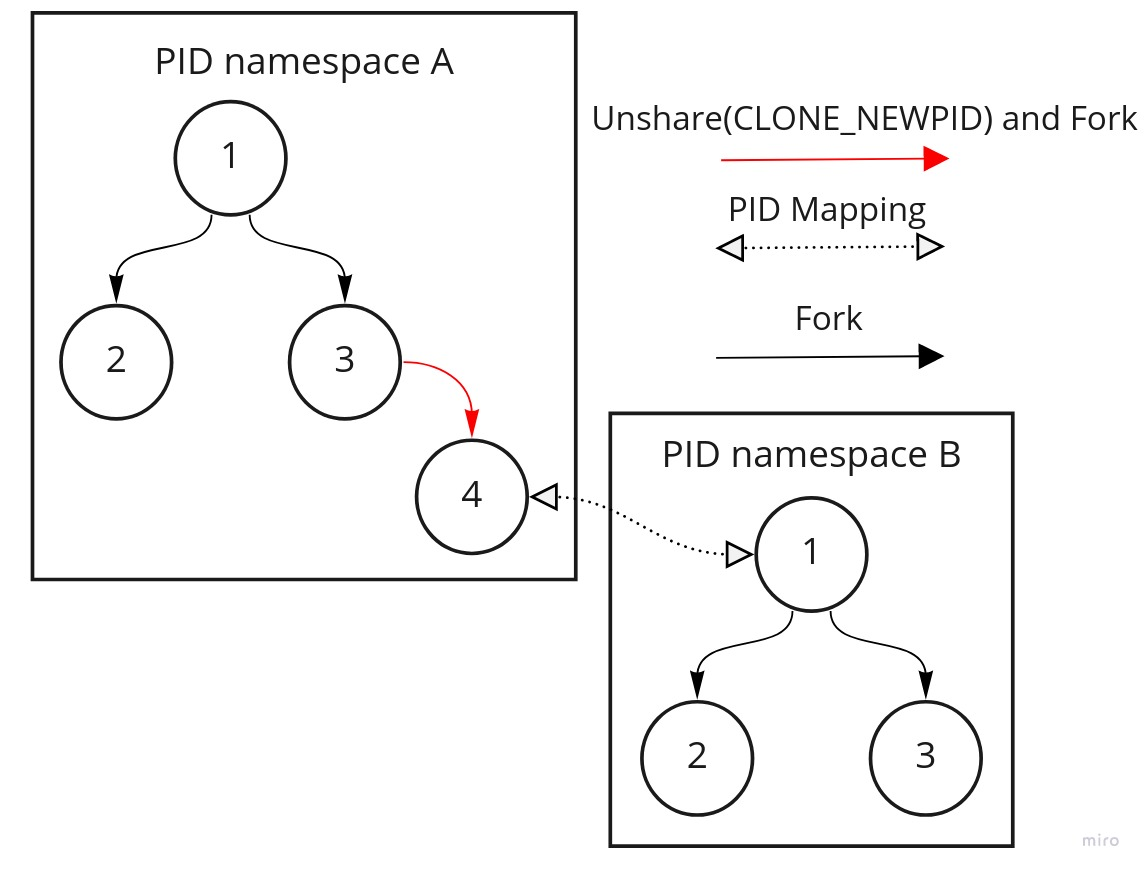
\includegraphics[width=0.55\textwidth]{images/fundamentals/pid-namespace-hierarchy.jpg}
    \caption{PID namespace hierarchy}
    \label{images:fundamentals/pid-namespace-hierarchy.jpg}
\end{figure}
Process identiifer (PID) namespaces encapsulate the mechanism of assigning 
unique identifiers to their resident processes. Every PID namespace localises an associative 
array, called the identifier registry, capable of allocating up to $2^{22}$ unique numbers and mapping them to arbitrary 
pointers. Because of this localisation, processes in different namespaces can be mapped to the 
same identifier. The first process to join a PID namespace receives the process identifier $1$ 
and acts as the init process for the entire namespace. This process becomes the parent of 
any orphaned children inside the namespace. Furthermore, if the init process terminates, all processes 
in the namespace terminate as well. In this case, even if a file descriptor to the namespace is kept open, 
i.e the namespace is kept alive by the kernel, no process is allowed to join.  

Process identifier namespaces are organised into a hierarchy, 
as shown by Figure \ref{images:fundamentals/pid-namespace-hierarchy.jpg}.
When a process calls \verb|unshare| with the \verb|CLONE_NEWPID| flag set, 
the kernel does not detach the process into a new PID namespace. Doing so would require 
changing the identifier of the process.
Instead, the kernel caches the new namespace in the process's namespace proxy and 
spawns the process's future children into it. The new process namespace is accessible from 
user-space via the \verb|/proc/[pid]/ns/pid_for_children| file. 

We denote $N_{i}$ as the $i$-th process in namespace $N$. 
In Figure \ref{images:fundamentals/pid-namespace-hierarchy.jpg},
$A_{1}$ forks two children $A_{2}$ and $A_{3}$. 
$A_{3}$ calls \verb|unshare| and registers a new PID namespace in the kernel. The process 
subsequently forks $A_{4}$, which the kernel translates into $B_{1}$.
Note that $A_{1}$ and $A_{2}$ can, by definition, interact with $B_{1}$ because $B_{1} = A_{4}$.  
Hence, a process is visible to all of its peers in its namespace and to all direct ancestor
namespaces. Conversely, $B_{2}$ and $B_{3}$ cannot see any processes in $A$. 
Joining a PID namespace is an irrevirtible operation, i.e if $A_{2}$ joins $B$,
then it cannot go back.

PID namespaces can be nested arbitrarily up to 32 times. 
Container runtimes do not utilise this feature, because application workloads are orthogonal 
to each other. Nesting two application workloads, potentially stemming from two different tenants, in a hierarchy
would enable processes resident in the ancestor namespace to kill the init process of the child namespace, which 
is in direct conflict with the noninterference property. 

\begin{lstlisting}[style=c-code-snippets, label={code:fundamentals/namespaces/process}, caption={PID namespace creation pseudocode}]
/* pid_namespace.c */
int err = unshare(CLONE_NEWPID);
pid_t child = fork();
if (child == 0) 
    child = fork();
    if (child == 0)
        execlp("sleep", "sleep", "60", (char *) NULL);
    else if (child > 0)
        exit(waitpid(child, NULL, 0) != child);
else 
    return waitpid(child, NULL, 0) != child;
\end{lstlisting}

Code snippet \ref{code:fundamentals/namespaces/process} demonstrates the creation of a new 
PID namespace with two processes. On lines 1 and 2, a new 
pid namespace is created through the \verb|unshare| system call and its init process is forked. 
The init process creates a new child that sleeps for 60 seconds. All processes within this 
hierarchy await their children's completion. 
We can run this example in a shell and list the shell's children via the \verb|ps|
utility, as shown in Code snippet \ref{code:fundamentals/namespaces/process-cmd}. 
You'll notice that the \verb|sleep| command is visible from the ancestor namespace and can be killed,
i.e directly interfered with. 
\begin{lstlisting}[label={code:fundamentals/namespaces/process-cmd}, style=bash, caption={Example of creating a PID namespace and listing all processes in the child namespace from a process in the parent namespace}]
$ ./pid-namespace &
[1] 78972
$ ps
PID TTY TIME CMD
62983 pts/1 00:00:00 bash
78972 pts/1 00:00:00 pid-namespace
78973 pts/1 00:00:00 pid-namespace
78974 pts/1 00:00:00 sleep
79027 pts/1 00:00:00 ps
\end{lstlisting}

%This has several implications. First, 
%this process becomes the parent of any orphaned children.
%If it fails to reap a child, the kernel will not release the child's process identifier from 
%the namespace identifier registry. Cumulatively pilling up the reserved identifiers may 
%result in the inability to spawn new processes. Second, if the init process terminates, all 
%processes in the namespace are terminated as well. 

%The noninterference boundary of a PID namespace heavily relies on the correct operation of the 
%init process. To prevent a member of the PID namespace from killing the init process and therefore 
%interfering with its peers, the kernel only propagates signals for which the init process 
%has established handlers for. 

\subsection{Mount Namespace}
\label{sections:fundamentals/namespaces/mount}
Files are multiplexed across multiple devices, each with its own intrinsic implementation details 
for storing and managing data. The kernel abstracts the underlying idiosyncrasies 
by arranging all files into a hierarchy that can be accessed through a well-defined programming interface. 
The process of attaching a device's file system 
to this hierarchy is called \textit{mounting}. The position in the hierarchy where the file system 
is attached is referred to as a \textit{mount point}.

Mount namespaces encapsulate the list of mount points that their resident processes can 
see. When a process detaches into a new mount namespace, it inherits an exact replica of the parent's mount points.
This does not necessarily mean that a change made by the parent to an underlying mount point remains 
invisible to the child, or vice versa. Every mount point is associated with a dedicated \textit{propagation type} 
that determines whether or not file system events are shared across mount namespaces 
that reference it. In essence, the propagation types governs the file system's noninterference boundary.

\subsection{Network Namespace}
\label{sections:fundamentals/namespaces/network}

\subsection{Inter-process Communication Namespace}
\label{sections:fundamentals/namespaces/ipc}

\subsection{Time Sharing Namespace}
\label{sections:fundamentals/namespaces/uts}

\subsection{Control Group Namespace}
\label{sections:fundamentals/namespaces/cgroups}

\section{Extended Berkley Packet Filters (eBPF)}
\label{sections:fundamentals/ebpf}